\documentclass[12pt]{article}
\usepackage[french]{babel}
\usepackage{natbib}
\usepackage{url}
\usepackage[utf8x]{inputenc}
\usepackage{amsmath}
\usepackage{graphicx}
\usepackage[svgnames]{xcolor}
\usepackage{vmargin}
\setmarginsrb{3 cm}{1 cm}{3 cm}{1.5 cm}{1 cm}{0.5 cm}{1 cm}{1.5 cm}
\usepackage{multirow}
\graphicspath{{images/}}
\usepackage{parskip}
\usepackage{fancyhdr}
\usepackage[T1]{fontenc}
\usepackage{url}
\usepackage{pdfpages}
\usepackage{url}
\usepackage{hyperref}
\usepackage{graphicx}

\usepackage{subfigure}
\usepackage{caption}

\usepackage{subcaption}
\usepackage{empheq, cases}
\usepackage{amssymb}
\usepackage{amsmath}
\usepackage{verbatimbox}
\usepackage{tcolorbox}
\usepackage{float}
\usepackage{multicol}
\usepackage[compact]{titlesec}
\usepackage[colorinlistoftodos]{todonotes}






\xdefinecolor{gray}{named}{lightgray}
\xdefinecolor{alice}{named}{AliceBlue}
\xdefinecolor{saumon}{named}{PeachPuff}
\definecolor{myred1}{RGB}{255, 0, 0}
\definecolor{mygreen1}{RGB}{0, 126, 0}
\definecolor{myblue1}{RGB}{0, 0, 61}
\definecolor{lightgray}{rgb}{0.83, 0.83, 0.83}
\definecolor{brick}{rgb}{0, 0, 0.50}

\tcbset{colback=lightgray,colframe=black}



\title{\color{brick} Optimisation TD 2:\\
\LARGE{Régression non linéaire et méthode de levenberg Marquardt}}								% Title
\author{Émilie Mathian}								% Author
\date{Année 2018 - 2019}											% Date

\makeatletter
\let\thetitle\@title
\let\theauthor\@author
\let\thedate\@date
\makeatother

\pagestyle{fancy}
\fancyhf{}
\rhead{\theauthor}
\lhead{Optimisation TD 1}
\cfoot{\thepage}
%%%%%%%%%%%%%%%%%%%%%%%%%%%%%%%%%%%%%%%%%%%%%%%%%%%%%%%%%%%%%%%
\usepackage{eso-pic}
\newcommand\BackgroundPic{%
\put(0,0){%
\parbox[b][\paperheight]{\paperwidth}{%
\vfill
\centering
\includegraphics[width=\paperwidth,height=\paperheight,%
keepaspectratio]{background.png}%
\vfill
}}}
  
  
\begin{document}

%%%%%%%%%%%%%%%%%%%%%%%%%%%%%%%%%%%%%%%%%%%%%%%%%%%%%%%%%%%%%%%%%%%%%%%%%%%%%%%%%%%%%%%%%

\begin{titlepage}
	\centering
    \vspace*{0.5 cm}
    \vspace{-3.5cm}
    
\includegraphics[width = 4cm]{logo.png}\\	% University Logo
    \textsc{\LARGE Institut National des Sciences Appliquées de Lyon}\\[2.0 cm]	% University Name
	\textsc{\Large $4^{eme}$ Année Bioinformatique et Modélisation}\\[0.5 cm]				% Course Code
	\textsc{\large Professeur: Noëlie DEBS }\\[0.5 cm]				% Course Name
	\rule{\linewidth}{0.2 mm} \\[0.4 cm]
	{ \huge \bfseries \thetitle}\\
	\rule{\linewidth}{0.2 mm} \\[1.5 cm]
	
	\begin{minipage}{0.4\textwidth}
		\begin{flushleft} \large
			\emph{Auteur:}
			\theauthor
			\end{flushleft}
			\end{minipage}~
			\begin{minipage}{0.4\textwidth}	
	\end{minipage}\\[2 cm]
    \vspace{-1.8cm}
	 \begin{figure}[H]
	\begin{center}
	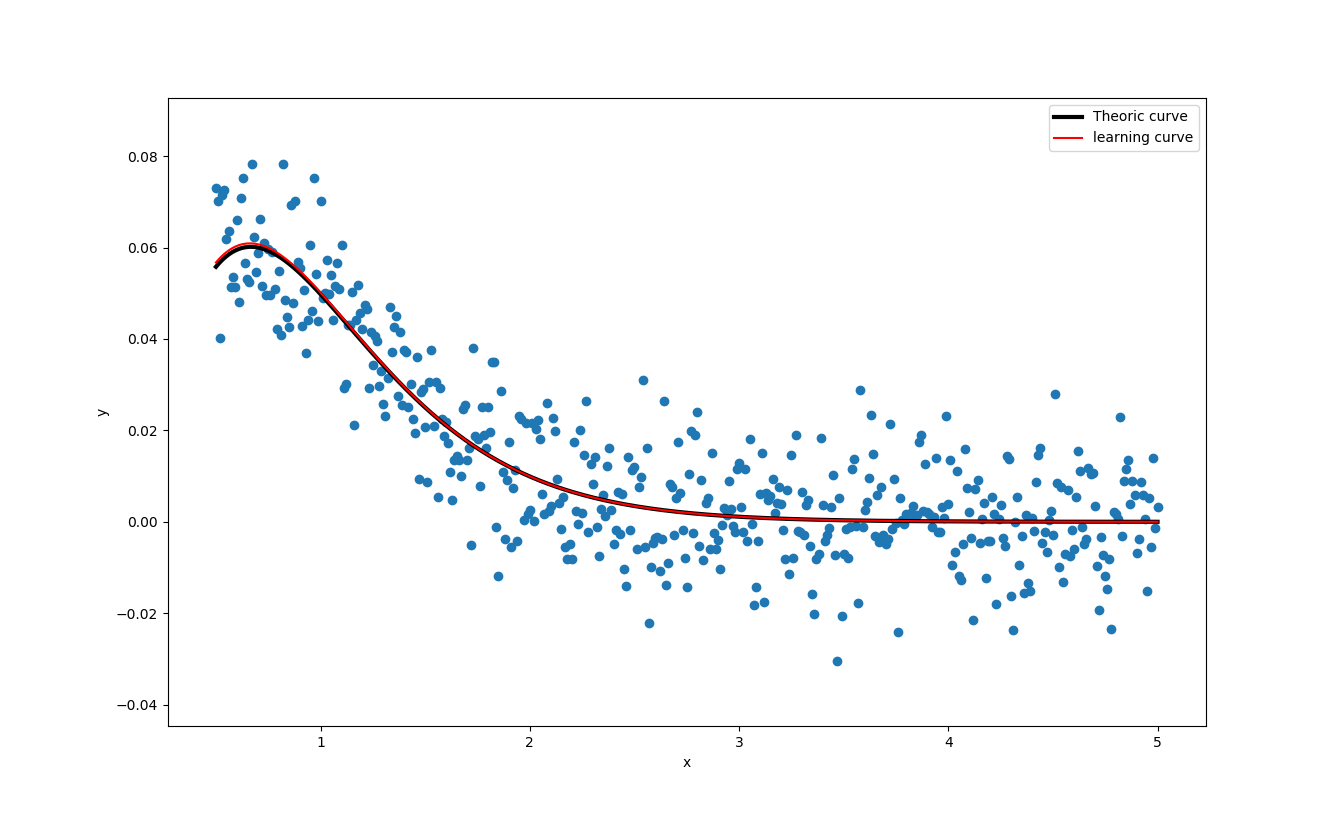
\includegraphics[width=0.9 \textwidth]{Figure_1.png}
\end{center}
\end{figure}

	{\large \thedate}\\[1 cm]
    
	\vfill

 

\end{titlepage}
\pagebreak
%%%%%%%%%%%%%%%%%%%%%%%%%%%%%%%%%%%%%%%%%%%%%%%%%%%%%%%%%%%%%%%%%%%%%%%%%%%%%%%%%%



\newpage 


\newpage

\begin{center}
\fcolorbox{black}{lightgray}{
\begin{minipage}{\linewidth}
\textbf{Problématique :} \\
L'objectif de ce TD est d'implémenter la méthode de Levenberg Marquardt. Cet
algorithme, dans le contexte de la régression non linéaire, permet  d'obtenir une estimation optimale des paramètres de l'équation du modèle telle que la somme des carrés des écarts soit minimisée. L'ensemble du programmme est contenu dans le fichier "TP2\_opt.py", les questions sont référencées dans le "Main" du programme. \\
\textit{Nb : les normes sont calculées d'après la définition de normes euclidiennes telles que $||\vec{u}||= \sqrt{x^2 + y^2}$}
\end{minipage}}
\end{center}
\vspace{0.5cm}

\section*{\color{brick} Cas 1:  Fonction mono exponentielle}
\textbf{\color{brick}1.} 
Dans le TP précédent nous avions implémenté la méthode de descente de gradient, et nous avions constaté que cet algorithme est performant dans le sens où il garantit de minimiser à chaque itérations la fonction de coût. Néanmoins la méthode de descente de gradient impose de fixer un pas de converge $\alpha$ tel que $f(x_k+1) = f(x_k) - \alpha \nabla f $, il sera donc laissé à l'utilisateur le soin d'optimiser le choix de ce paramètre. De plus cette méthode impose que $f$ soit de classe $\mathcal{C}^1$. Enfin malgré sa facilité à être implémentée elle reste une méthode peu efficace ayant une faible vitesse de convergence.\\
L'implémentation de la méthode de Newton nous a permis d'observer l'efficacité de l'algorithme étant donné sa vitesse de converge. Toutefois, l'algorithme de Newton ne distingue pas les maximums des minimums ni les points selle. De plus la méthode repose sur le calcul de la Hessienne, calcul coûteux qui impose que $f$ soit de classe $\mathcal{C}^2$, enfin cette matrice Hessienne doit être définie positive.\\

\textbf{\color{brick}2.} La fonction g a pour expression : $g(x) = e ^{-ax}$. Le seul paramètre que nous devrons estimer est donc '$a$'. Le calcul de la fonction g a été implémenter avec \verb|g (x,a)|, où les entrées sont : \verb|x| un vecteur de dimension $(n,1)$, et \verb|a| une valeur pour le paramètre à estimer; la sortie est un vecteur \verb|y| de dimension $(n,1)$. \\


\textbf{\color{brick}3.} La fonction \verb|random_data_set(x,a,b)| permet de construire un jeu de données aléatoires de y points tels que  $y= g(a,x) +b \mathcal{N}(0,1)$. Ainsi pour tout x on calcul le résultat de la fonction $g(x)$ auquel on ajoute un résidu aléatoire tiré d'une loi normale centrée réduite que l'on pondère d'un facteur $b$.
\newpage

\textbf{\color{brick}4.} 
\begin{figure}[H]
\centering
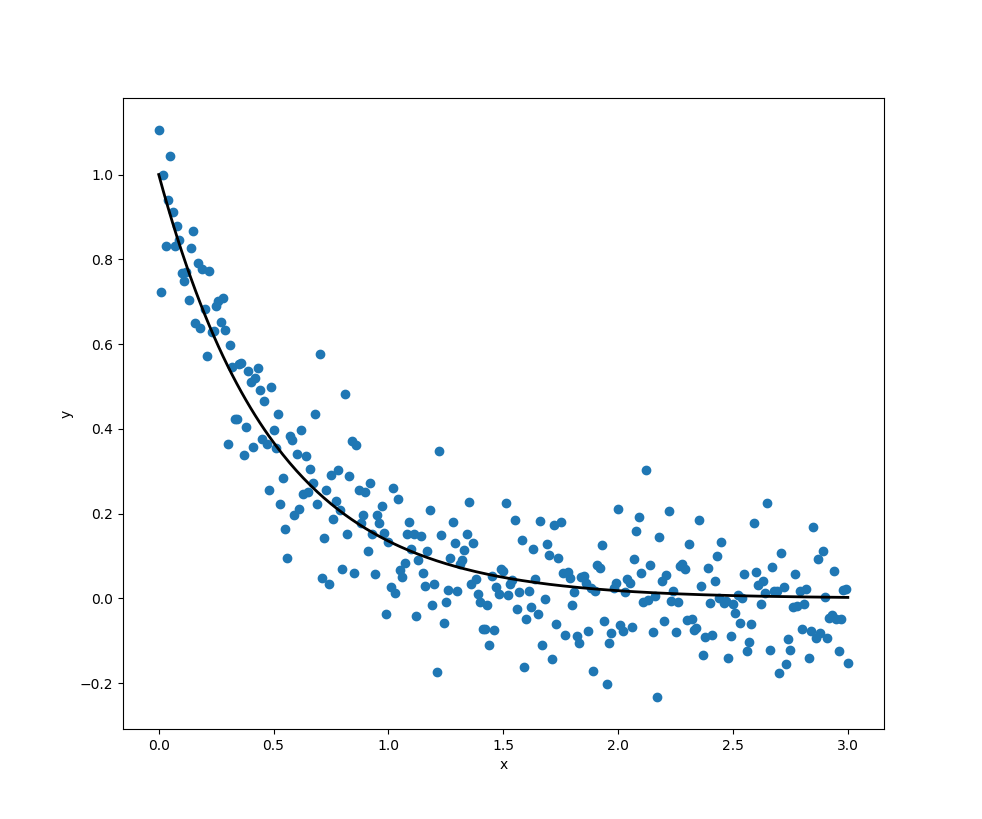
\includegraphics[width=0.6\textwidth]{Q4.png}
\caption{Génération d'un jeu de données aléatoire tel que $y= e^{-2x} + b \mathcal{N}(0,1) $ avec b=0.1, sur un intervalle $x\in[0,3]$. La courbe noir a pour équation $y= e^{-2x}$, c'est donc par construction la fonction qui explique un plus ou moins grande part de la SCE selon le bruit. }
\label{Fig1}
\end{figure}

\textbf{\color{brick}5.} La fonction de coût à minimiser, dans le cas d(un modèle de régression non linéaire n'est autre que la fonction de la somme des carrés des écarts entre les données et le modèle. Cette fonction notée $f$ s'écrit alors  pour notre cas telle que $f(a) =\frac{1}{2}\sum_{i=1}^N(y_i - e^{-ax}) $.  Dans notre programme cette fonction a été nomée \verb|cost_fucntion(x,y,a)|, qui d'après un vecteur de données $y$, un vecteur $x$ et selon un paramètre $a$ retourne la SCE.


\textbf{\color{brick}6.} La minimisation de la fonction $f$ d'après la méthode de Levenberg Marquardt utilise le gradient de la fonction de coût. La formule général du gradient est \\
$\frac{\partial f}{\partial a_k} = - \sum_{i=1}^N = (y_i - g(x_i,a))\frac{\partial g}{\partial a_k}(x_i,a) $  ce qui dans notre cas donne :
$$ \frac{\partial f}{\partial a} =\sum_{i=1}^N (y_i - e^{-ax_i}(x_ie^{-ax_i})) $$
Ainsi nous avons écrit la fonction \verb|grad (x,y,a)|, qui prend en entrée le vecteur des données $y$ et un vecteur $x$ et un paramètre $a$  et retourne la valeur de la dérivée en fonction de $a$.
 
\textbf{\color{brick}7.} La méthode de Levenberg Marquardt requiert également le calcul de la dérivée seconde, nous utiliserons ici l'approximation de Gauss Newton pour simplifier les calculs. Rappelons que la formule générale est $\frac{\partial ^2 f }{\partial a_K \partial a_l} = \sum_{i=1}^N \frac{\partial g}{\partial a_k}g(x_i, \textbf{a})\frac{\partial g}{\partial a_l}g(x_i, \textbf{a})$, d'après notre fonction et sachant que nous n'avons qu'un paramètre à estimer nous obtenons :\\ 
\begin{align*}
    \frac{\partial ^2 f }{\partial a ^2} &=  \sum_{i=1}^N \frac{\partial g}{\partial a}g(x_i, a)\frac{\partial g}{\partial a}g(x_i, a)\\
    &= \sum_{i=1}^N ( \frac{\partial g}{\partial a}(x_i, a)^2) \\
    &=  \sum_{i=1}^N (-xe^{a-x})^2
\end{align*}
La fonction \verb|derivative_2 (x,a,l)| résoud l'opération ci-dessus; rappelons que l'algorithme de Levenberg Maquardt permet de moduler l'importance de la dérivée seconde par rapport à la dérivée première en multipliant $ \frac{\partial ^2 f }{\partial a ^2} $ par un coefficient $(1+ \lambda)$, c'est pourquoi  \verb|derivative_2| prend en entré le paramètre \verb|l| qui traduit $\lambda$. La fonction  retourne pour un $a$ et un $\lambda$ donnés le résultat de la dérivée seconde de la fonction de coû.

\textbf{\color{brick}8.} Implémentation de l'algorithme de Levenberg Maquardt :\\
L'algorithme  est nommé \verb|LM| pour le premier cas, il prend en entré les paramètres suivants :
\begin{itemize}
    \item \verb|x| un vecteur définissant l'intervalle de l'analyse
    \item \verb|y| un vecteur de données aléatoires (généré par \verb|random_data_set|)
    \item \verb|a| l'estimation initiale du paramètre
    \item \verb|l| une condition initiale du paramètre $\lambda$, coefficient modulant l'importance du gradient par rapport à la Hessienne lors du calcul de la direction.
    \item\verb|cond| qui est la condtition d'arrêt choisit qui d'après la fonction \verb|stop| peut les veleurs suivantes :
    \begin{itemize}
        \item 0 => condition d'arrêt par  rapport à un nombre maximal d'itérations donné par le paramètre \verb|k|
        \item 1 => condition d'arrêt par rapport à une norme minimale à atteindre donnée par le paramètre \verb|g|
        \item 2 => conditions d'arrêt reliant le nombre d'itérations maximal et la norme minimale à atteindre
        \item 3 => condition d'arrêt impliquant que l'inéquation $f(a_{k+1})<f(a_k)$ soit vérifiée.
    \end{itemize}
\end{itemize}

À chaque itération l'algorithme \verb|LM| retourne la dernière  valeur de  $a$, la norme du gradient (\textit{ici équivalente à la valeur absolue de la dérivé première}), la fonction de coût dépendante de la dernière valeur calculée de $a$ dépendant et la valeur de $a$ depnedant elle même la direction calculée, notée \verb|dLM|. Rappelons en effet que  \verb|dLM|  est calculée telle que $dLM = -\frac{\nabla}{\nabla^2 f (1 + \lambda)}$ et que sa mise jour implique que  $a_{k+1} = a_k +dLM$. Soulignons par ailleurs que la mise jour de $a$ et $\lambda$ par rapport à \verb|dLM| dépend de vérification  de la condition $f(a_{k+1}) < f(a_k)$.

\textbf{\color{brick}9.} Nous allons étudier le comportement de l'algorithme \verb|LM| pour chaque itérations, avec les paramètres $g(x)= e{-2x}$ (d'où $a=2$) sur $x \in [0,3]$ et $b=0.01$.

\begin{figure*}
  \centering
  \subfigure[Dynamique Oscillante]{%
    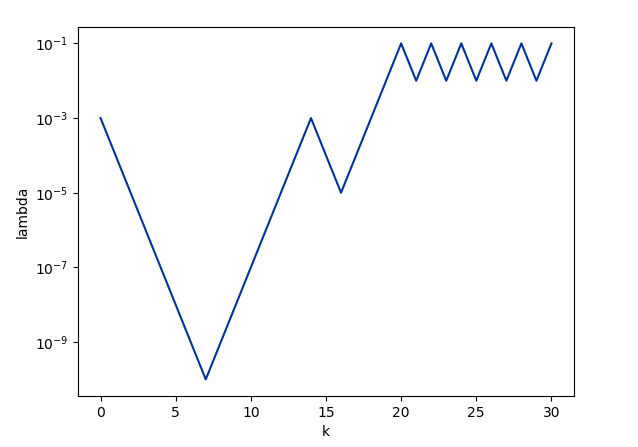
\includegraphics[width=0.45\textwidth]{Q9_oscillation.png}
    \label{fig:a}%
    }%or more
    \subfigure[Dynamique 'explosive']{%
    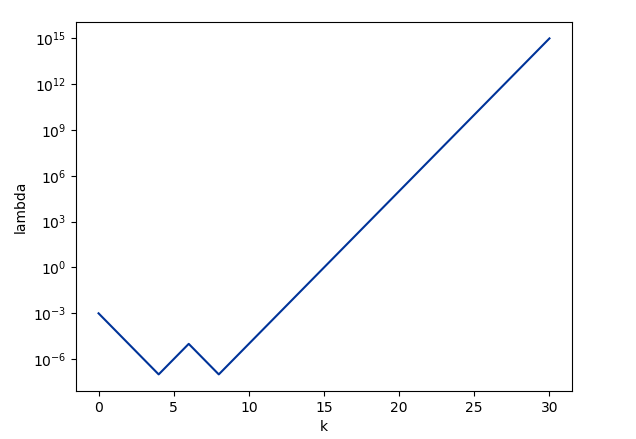
\includegraphics[width=0.45\textwidth]{Q9_Explose.png}
    \label{fig:b}%
  }%  
  \caption{Dynamique de $\lambda$}
  \label{fig:ab}
\end{figure*}




La dynamique de $\lambda$ est très variable, l'évolution de $\lambda$ peut ainsi exploser en fin processus [\ref{fig:b}], ou bien osciller  [\ref{fig:a}]. Toutefois pour des valeurs de bruit 'raisonnables' les valeurs en $\lamda$ suivent un schéma,  ainsi nous pouvons généraliser :\\
En début du processus $\lambda$ est faible alors :\\
pour $H_{LM}$ qui dans cet exemple équivaut $\frac{\partial^2 f}{\partial a^2}(1+\lambda)$ on a :
$$\lim_{\lambda\to 0} H_{LM} = \frac{\partial ^2f}{\partial a^2} $$
d'où $d_{LM} \simeq -\frac{\nabla f}{\nabla^2f}$
Ainsi pour les premières itérations l'algorithme de Levenberg Maquardt suit la méthode de Newton. \\
En fin de processus les valeurs de $\lambda$ peuvent exploser alors :
$$\lim_{\lambda\to +\infty} \frac{\partial ^2 f}{\partial a^2}(1+\lambda) = +\infty \Longleftrightarrow \lim_{\lambda\to +\infty} \frac{1}{\frac{\partial ^2 f}{\partial a^2}(1+\lambda)} = 0$$

d'où $$\lim_{\lambda\to 0} d_{LM} =\frac{\partial f}{\partial a} * \frac{1}{\lambda} $$
Ainsi dans un seond temps la méthode converge vers le gradient descente.\\
Parfois on peut observer une  dynamique oscillante de $\lambda$ représentant un usage alternatif des deux méthodes.\\


Observons à présent l'évolution de la norme du gradient :

\begin{figure}[H]
\centering
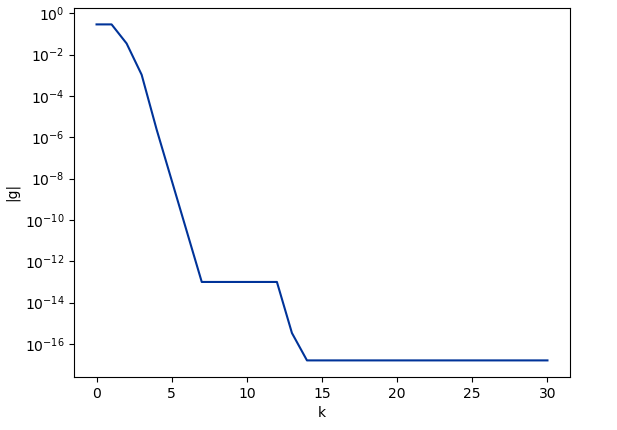
\includegraphics[width=0.5\textwidth]{GRAD_Q9.png}
\caption{ Évolution du logarithme de la norme du gradient $|g|$.}
\label{fig:ag}
\end{figure}

\begin{figure}[H]
\centering
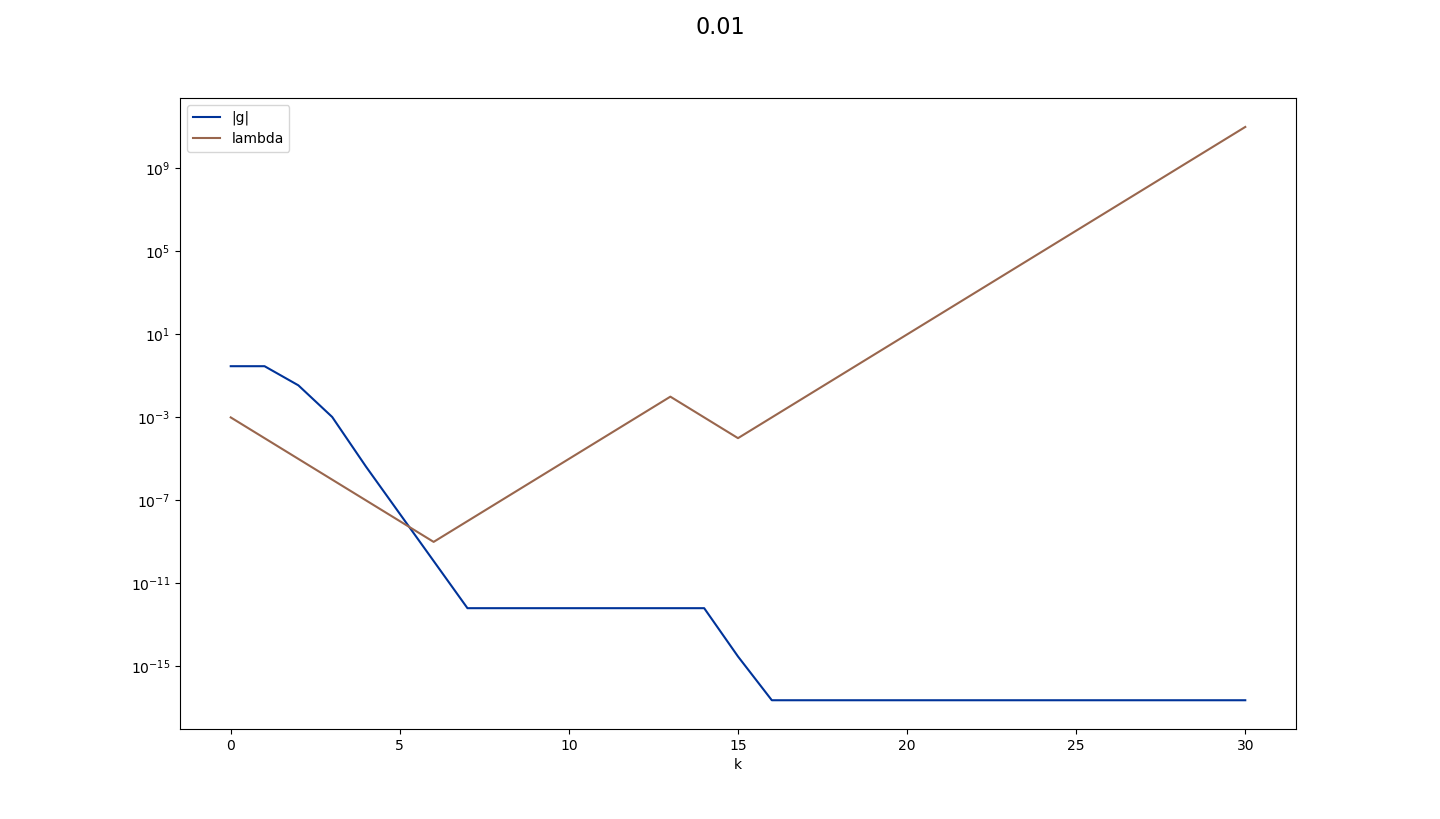
\includegraphics[width=0.7\textwidth]{COMP_GRAD_L.png}
\caption{ Évolution du logarithme de la norme du gradient $|g|$ et du logarithme de $\lambda$.}
\label{fig:ag2}
\end{figure} 


D'après la figure [\ref{fig:ag}], le gradient descend par paliers, nous pouvons remarquer d'après le figure [\ref{fig:ag2}] que les phases croissantes de $\lambda$ sont associées à des phases quasi stable de $\log(|g|)$ et pour des décroissante de $\lambda$ on aboutit à de fortes diminutions de $\log(|g|)$. Ainsi sur une échelle logarithmique nous pouvons observer que la vitesse de convergence de l'algorithme de Newton et bien supérieur à celle du gradient descente.

\begin{minipage}{0.5\textwidth}
D'après la représentation de la fonction de coût $f(x,a)$, au cours des itérations, nous observons que l'écart résiduel entre le modèle et les données  converge rapidement vers un minimum. 
Remarquons qu'ici pour la valeur du bruit est très faible $b=0.01$, ainsi la SCE  converge rapidement vers 0, ce qui ne serait pas le cas pour des données plus buritées.
\end{minipage} \hfill
\begin{minipage}{0.45\textwidth}
\begin{figure}[H]
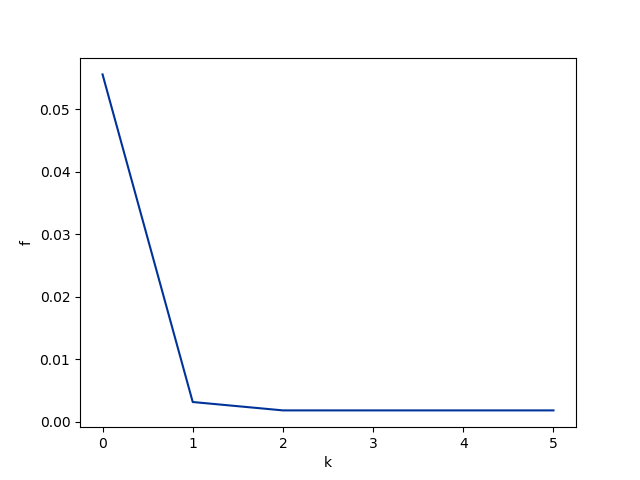
\includegraphics[width=1\textwidth]{Figure_5.png}
\caption{Évolution de la fonction de coût}
\label{Fig1}
\end{figure}
\end{minipage}


\textbf{\color{brick}10.} Nous étudions à présent  l'effet du paramètre $b$ sur la convergence de l'algorithme \verb|LM|. Pour cela nous fixons $a=2$, nous travaillons un intervalle tel que $x \in [0,3]$ et nous prenons différentes valeurs de bruits $b=[0.01, 0.1 , 0.5 , 1]$. Nous obtenons les résultats suivants : 
\begin{itemize}
    \item Si $b<1$ nous observons des résultats comparables à ceux précédents.
    \item Si b est grand alors les résultats sont aberrants
\end{itemize}


\begin{figure}[H]
\centering
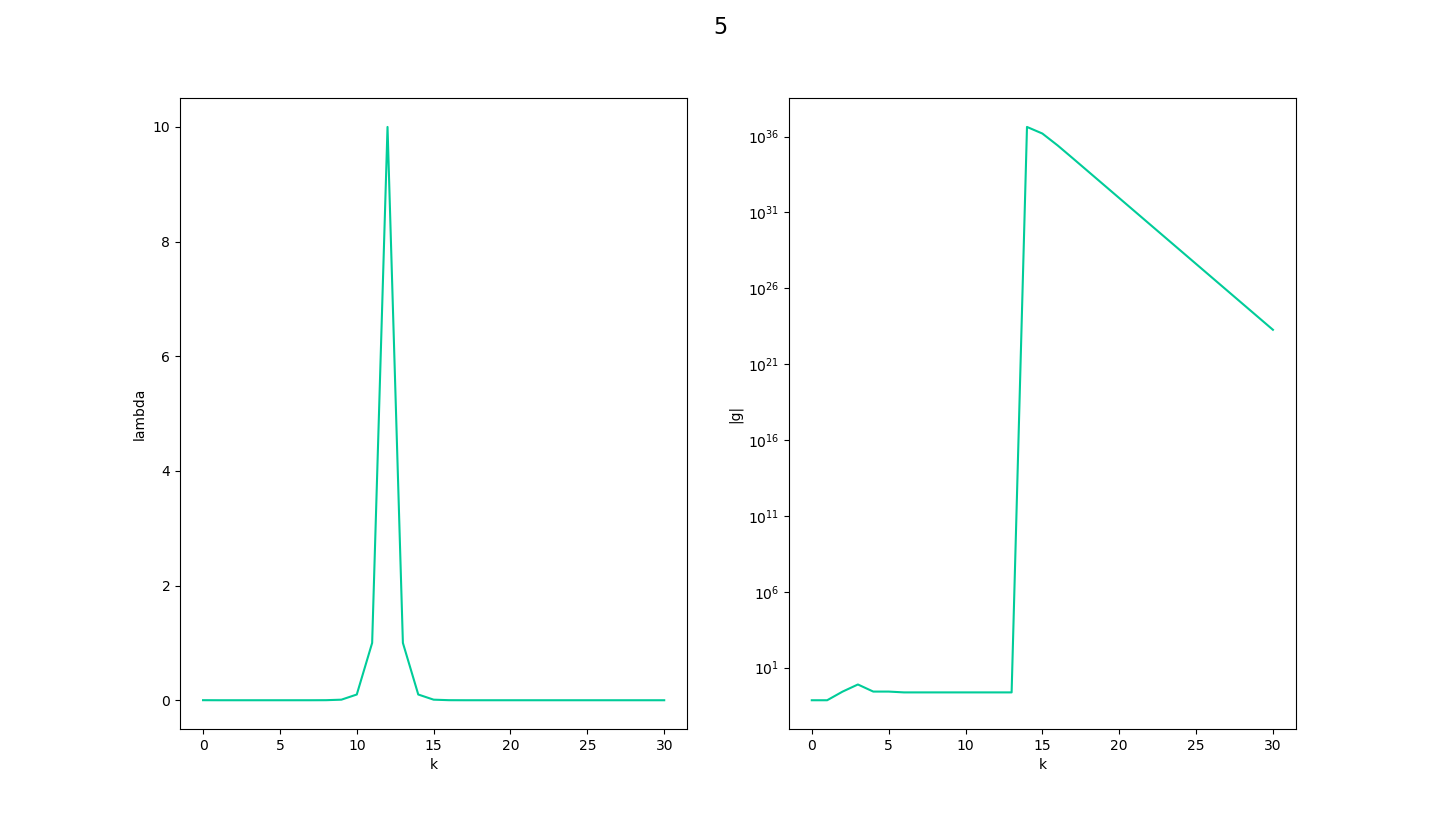
\includegraphics[width=0.6\textwidth]{Q10_Aberant.png}
\caption{ Évolution de $\lambda$ et de $|g|$ pour $b=5$. Nous observons des valeurs de $|g|$ aberrantes, de plus l'approximation l'est elle aussi avec $a=-8.379$}
\label{FigQ10}
\end{figure}

\begin{minipage}{0.45\textwidth}
D'après le graphique ci-contre, l'algorithme converge rapidement vers le minimum de la fonction de coût. Ensuite la SCE se stabilise  étant donné que $a$ devient quasi constant au cours des itérations. Par ailleurs l'augmentation du bruit induit comme attendu une augmentation globale de la SCE.

\end{minipage} \hfill
\begin{minipage}{0.5\textwidth}
\begin{figure}[H]
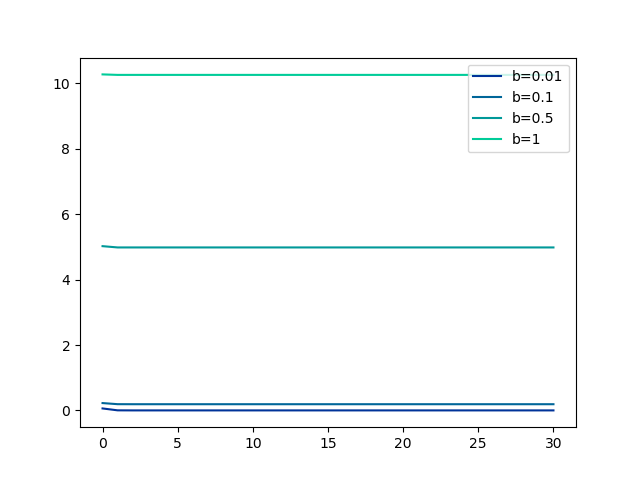
\includegraphics[width=0.7\textwidth]{Q10_F.png}
\caption{ Valeur de la fonction de coût en fonction du nombre d'itérations pour différentes valeurs de bruits.}
\label{FigQ10B01}
\end{figure}
\end{minipage}

Nous pouvons résumer l'influence du bruit avec  $b\in [0,0.3]$ en traçant l'évolution des différents paramètres du modèle en fonction de $b$, avec une condition d'arrêt fixée sur le nombre d'itérations (k<30).
\begin{figure}[H]
\centering
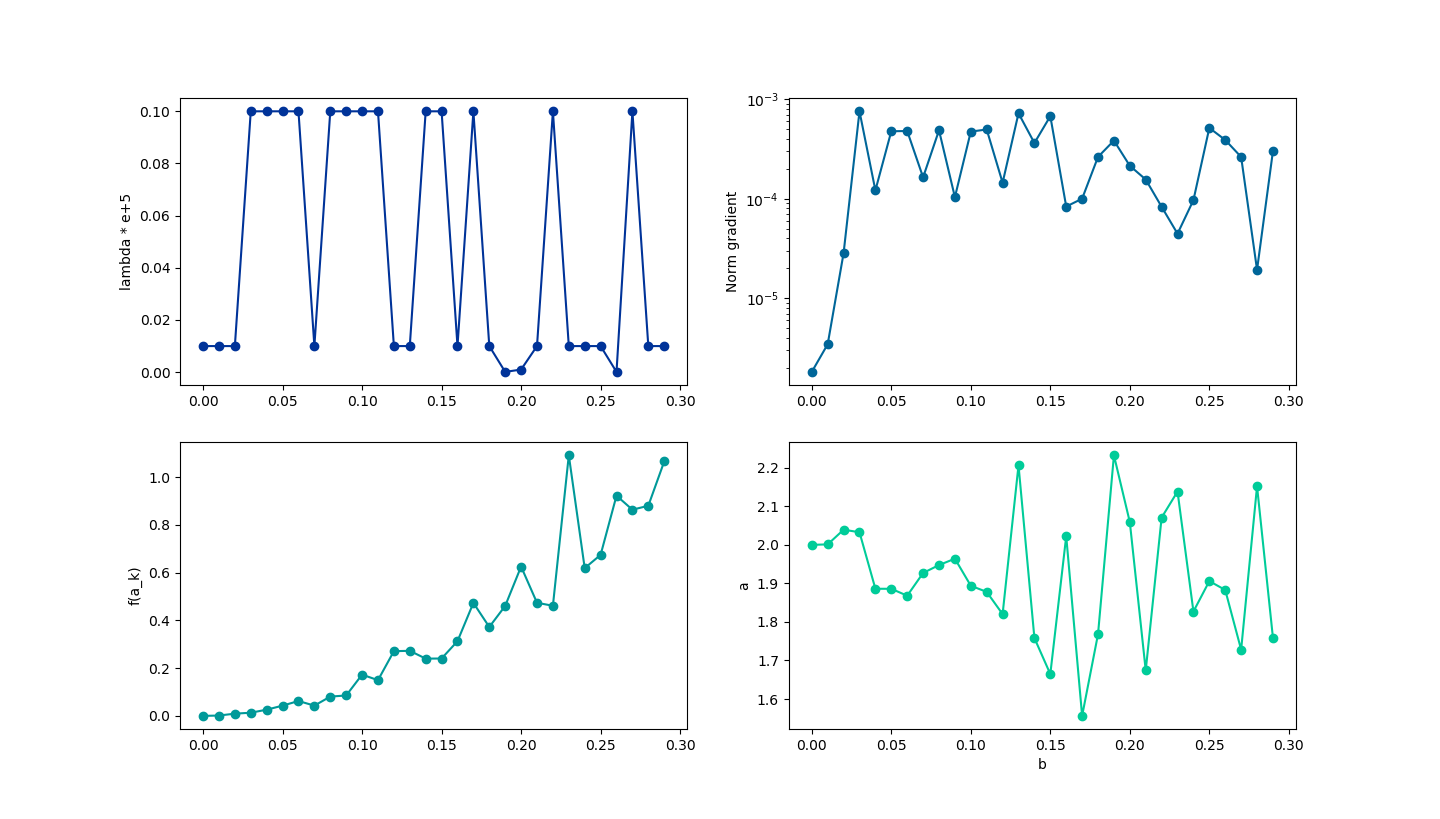
\includegraphics[width=1\textwidth]{Q10FF.png}
\caption{ Ébolution de $\lambda$, de $|g$, de $f(a_k)$ et de $a$ en fonction du bruit $b \in [0,0.3]$.}
\label{FigQ10B01}
\end{figure}
Ces graphiques résument les informations précédentes, en effet nous observons que comme attendu la SCE ($f(a)$ )croit avec le bruit, ou encore que la norme du gradient  reste faible mais croit et devient instable lorsque b augmente. Enfin nous observons que l'approximation de $a$ est très proche du $a$ théorique si $b$ est faible, puis oscille autour de la solution pour $b$ croissant.
\newpage

\textbf{\color{brick}11.} Nous allons à présents tracer les données et les prédictions pour différentes valeur de $b$ testées :

\begin{figure}[H]
\centering
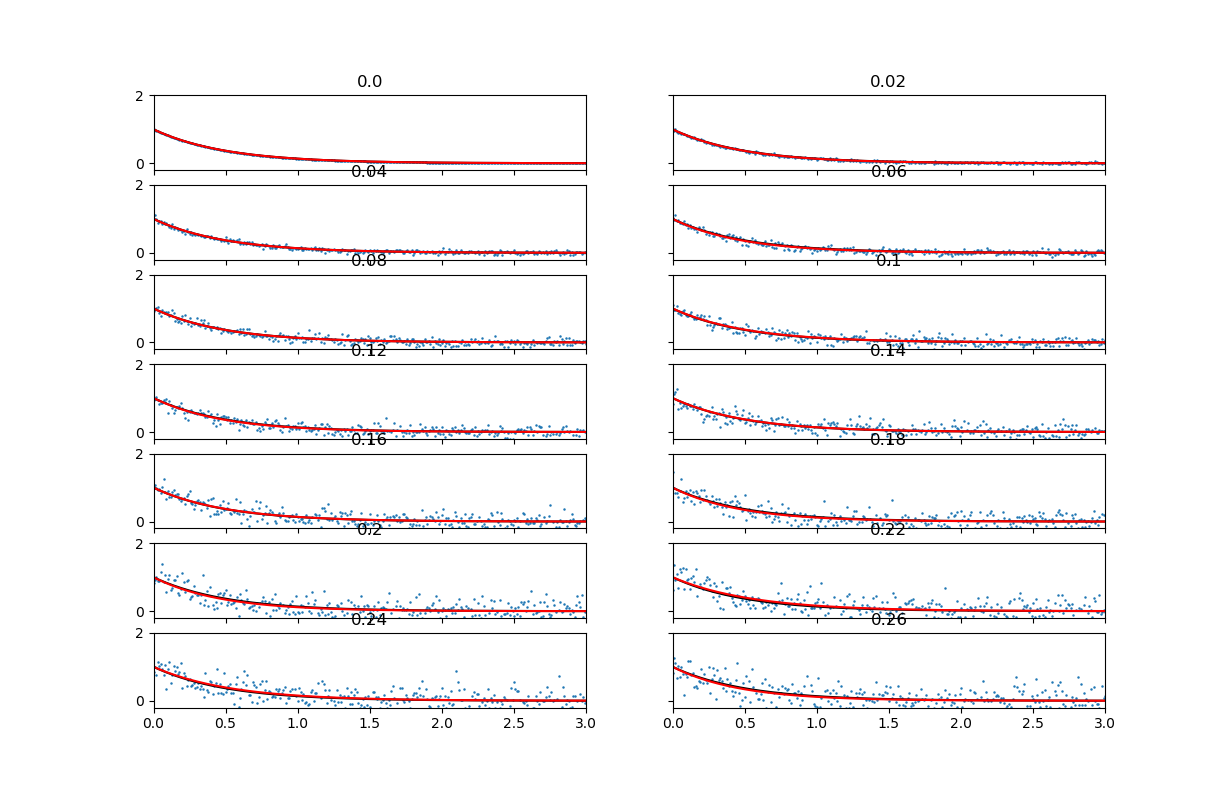
\includegraphics[width=1\textwidth]{Q111.png}
\caption{Données, courbe théorique (noire) et simulée (rouge) pour $a=2$ et différentes valeurs de $b  \in [0,3]$.}
\label{FigQ111}
\end{figure}

 D'après les graphiques ci-dessus [\ref{FigQ111}] la courbe calculée par la méthode de Levenberg Maquardt concorde parfaitement avec la courbe théorique. Par construction, lorsque $b$  est petit l'algorithme minimise donc l'écart aux données en s'ajustant sur le modèle théorique . Ainsi pour les valeurs de $b \in [0, 0.3]$ testées il est difficile de mettre en évidence visuellement une différence de la qualité de la modélisation en fonction du bruit. Nous devons donc essayer  des valeurs de $b$ supérieure pour observer une différence : 
 
 \begin{figure}[H]
\centering
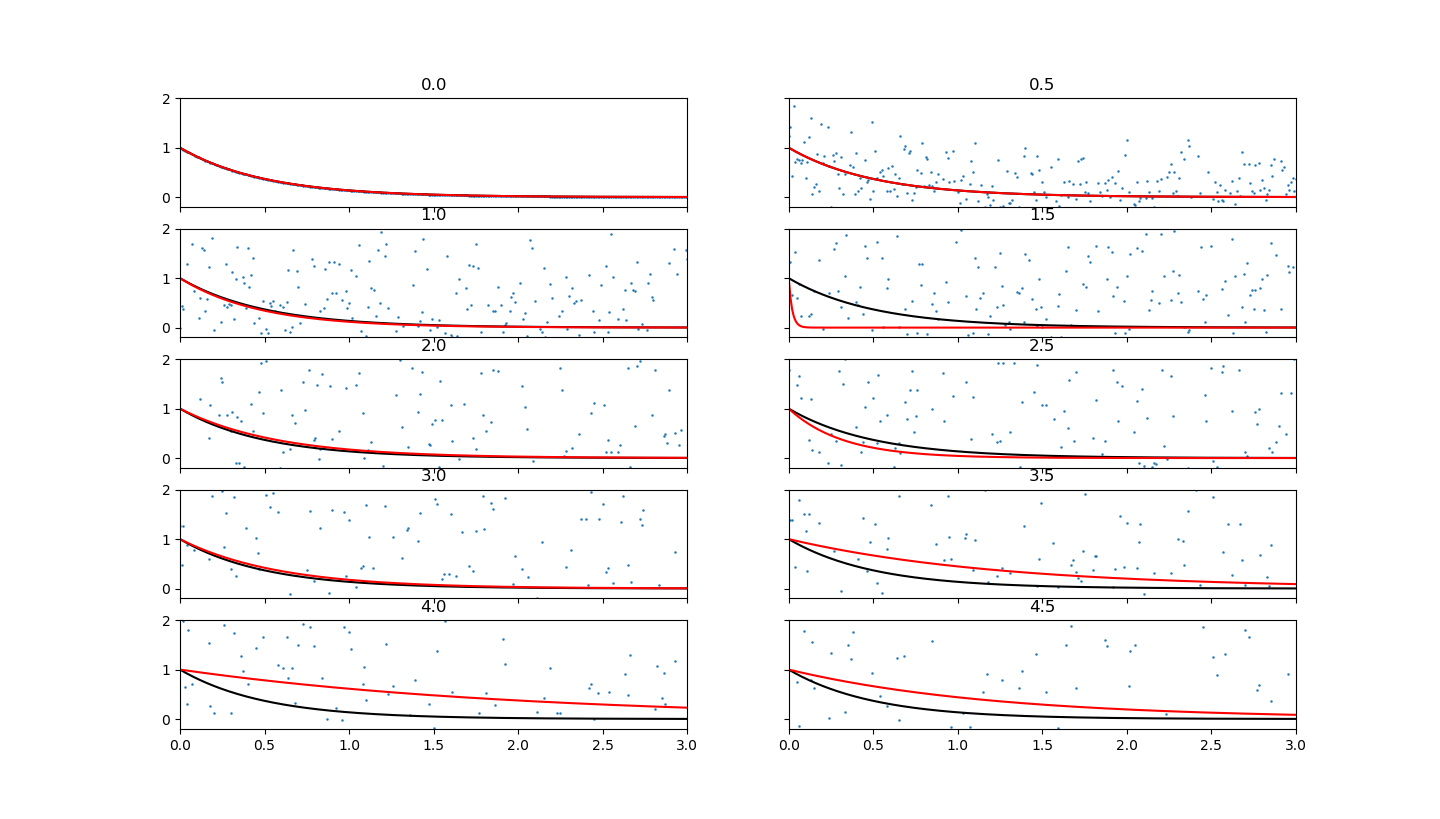
\includegraphics[width=1\textwidth]{Q1132.png}
\caption{Données, courbe théorique (noire) et simulée (rouge) pour $a_{th}=2$ et différentes valeurs de $b \in [0,5]$ par 0.5. Avec une condition d'arrêt fixée par rapport au nombre d'itérations et à la norme du gradient avec $k = 10000$ et $|g|=0.01$.}
\label{FigQ1132}


\end{figure}

On constate que pour $b$ supérieur à 1, la prédiction devient chaotique malgré une condition d'arrêt fixée sur le critère 2. Ce comportement est observé dans certains cas seulement. Ainsi le $a$ prédit peut être éloigné du $a$ réel et dans d'autre cas relativement proche du $a$ théorique (cas où $b = 4$). L'absence de converge vers le modèle théorique peut s'expliquer par  l'effet SCE à l'initiation et donc de  la distribution des $y_i$. En effet rappelons que $\frac{d f}{d a} = \sum_{i=1}^N (y_i - e^{-ax_i})(x e^{-ax_i})$, donc selon la distribution des $y_i$ la $dLM$ peut être fortement influencé, et l'estimation du paramètre $a$ rapidement biaisé. De plus la SCE augmente avec $b$. Toutefois cette seule explication n'est satisfaisante étant donné les résultats obtenus pour $b=1.5$ [\ref{FigQcap}] sont déjà aberrants. Il pourrait s'agir d'un défaut d'implémentation de l'algorithme \vreb|LM|.


  \begin{figure}[H]
\centering
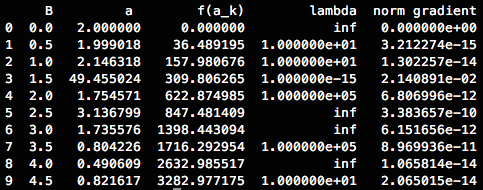
\includegraphics[width=1\textwidth]{Q113CAP.png}
\caption{Résultats numériques obtenu à la fin du processus pour les figures [\ref{FigQ1132}] .}
\label{FigQcap}
\end{figure}
 
 \section*{\color{brick} Cas 2:  Fonction bi-exponentielle}
 \textbf{\color{brick}1.} Nous travaillons sur la fonction $g(x) = x^a1 e^{-a2x}$. Comme précédemment les images $g$ sont renvoyés par la fonction \verb|g2(x,a1,a2)|, qui prend en entrée un vecteur \verb|x| et les valeurs des paramètres.\\
 Nous constituons un jeu de donnée à partir de cette fonction  $g(x)$ via la fonction \verb|random_data_set2(x,a1,a2,b)|  qui prend en entré  un vecteur x, dans l'exercice $x \in [0,5]$, les valeurs des paramètre ici $a1 = 2$ et $a2 =3$, et un bruit b, on prendra pour le test $b=0.01$.
 
 
  \begin{figure}[H]
\centering
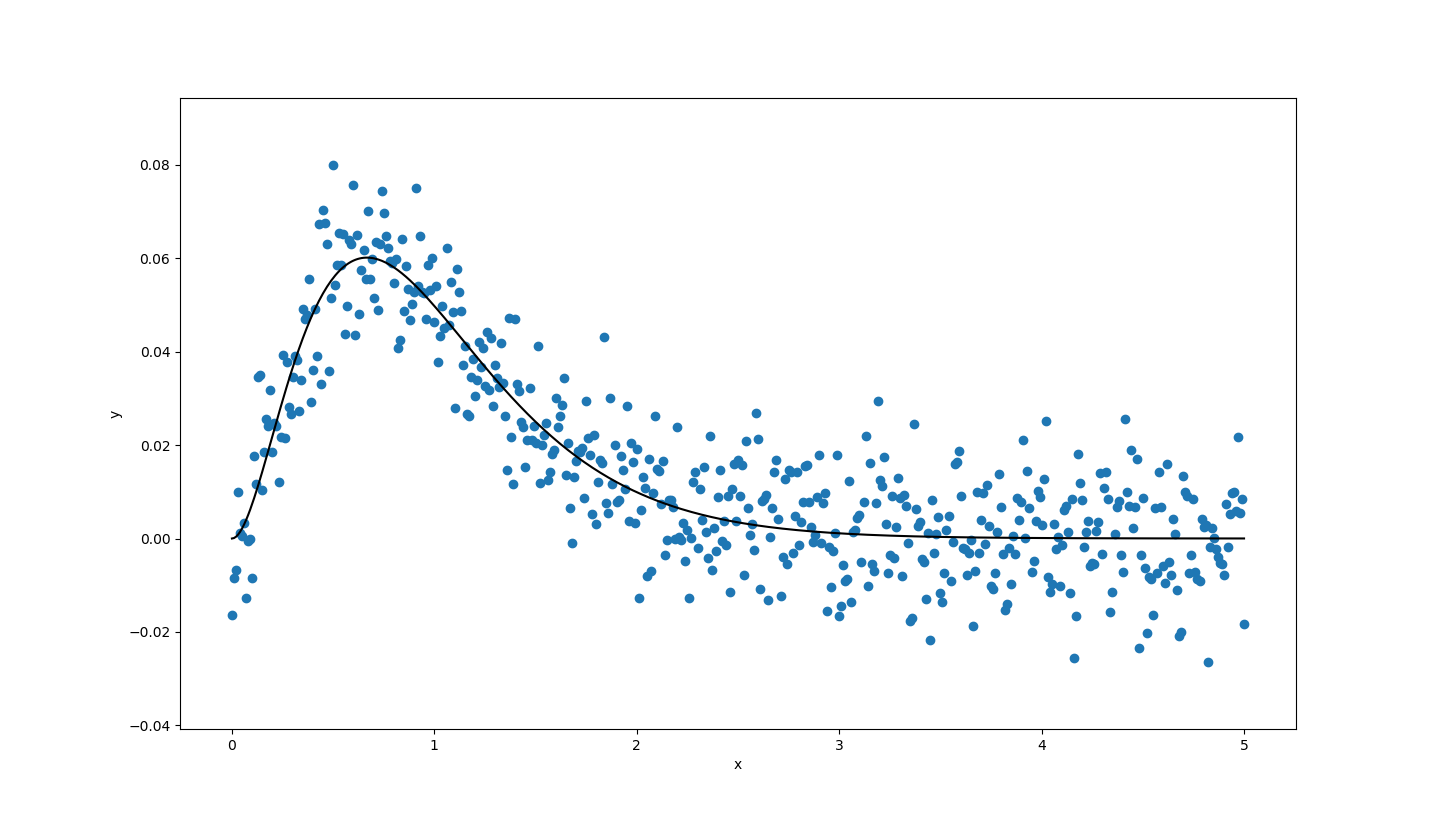
\includegraphics[width=0.7\textwidth]{Q12.png}
\caption{Représentation du jeu de données et de la courbe théorique $g(x)= x^{a1}e^{-a2x}$.}
\label{FigQ12}
\end{figure}

 \textbf{\color{brick}2 .} L'expression du gradient de $f$ par rapport à $a$ est :
 \begin{align*}
     \frac{\partial f}{\partial a1} &= -\sum_{i=1}^N (y_i - x_i^{a1}e^{-a2x})\frac{\partial g}{\partial a_1} \\
     &= -\sum_{i=1}^N (y_i - x_i^{a1}e^{-a2x})(ln(x)x^{a1}e^{-a2x})
 \end{align*}{}
  \begin{align*}
     \frac{\partial f}{\partial a2} &= -\sum_{i=1}^N (y_i - x_i^{a1}e^{-a2x})\frac{\partial g}{\partial a_2} \\
     &= -\sum_{i=1}^N (y_i - x_i^{a1}e^{-a2x})(-x^{a_1+1}e^{-a2x})
 \end{align*}{}
 
 Le gradient de la fonction f est donné par \verb|grad2 (x,y,a1,a2)| qui renvoie à partir d'un jeu de données contenues dans le vecteur \verb|y|, d'un intervalle \verb|x| et des deux paramètre, $\nabla f$, un vecteur de dimension 2.
 
 
  \textbf{\color{brick}3 .} Calculons la dérivée seconde de la fonction $f$ par rapport $a_1$ et $a_2$ :
  $$H = \begin{pmatrix} 
\frac{\partial^2 f}{\partial x^2} & \frac{\partial^2 f}{\partial x\partial y} \\
\frac{\partial^2 f}{\partial x \partial y} & \frac{\partial^2 f}{\partial y^2} \\
\end{pmatrix} =
\begin{pmatrix} 
\sum_{i=1}^N (ln(x) x^{a_1} e^{-a2x})^2 & \sum_{i=1}^N (ln(x) x^{a_1} e^{-a2x})(-x^{a_1+1}e^{-a2x})  \\
 \sum_{i=1}^N (ln(x) x^{a_1} e^{-a2x})(-x^{a_1+1}e^{-a2x}) & \sum_{i=1}^N (-x^{a_1+1}e^{-a2x})^2 \\
\end{pmatrix}
$$

Nous avons ici calculé la dérivée seconde par l'approximation de Newton. De plus dans notre cas nous allons multiplier la matrice Hessienne par $(1 + \lambda)$ pour favoriser les termes diagonaux si $\lambda$ est grand et donc l'importance de la dérivée première par rapport à la dérivée seconde et réciproquement si $\lambda$ est petit. On obtient :
$$HLM = 
\begin{pmatrix} 
\sum_{i=1}^N (ln(x) x^{a_1} e^{-a2x})^2 & \sum_{i=1}^N (ln(x) x^{a_1} e^{-a2x})(-x^{a_1+1}e^{-a2x})  \\
 \sum_{i=1}^N (ln(x) x^{a_1} e^{-a2x})(-x^{a_1+1}e^{-a2x}) & \sum_{i=1}^N (-x^{a_1+1}e^{-a2x})^2 \\
\end{pmatrix} (1 +\lambda)
$$
 
 Cette matrice est calculée grâce à la fonction \verb|derivative_2_f2(x,y,a1,a2, l)|, ici l représente la valeur de $\lambda$.
 
 \textbf{\color{brick}4 .}
Dans le cas bi-exponentielle la méthode de Levenberg Marquardt est contenu dans la fonction \verb|LM2 (x,y,a1, a2,l,cond, k, g)|. Cette fonction a les mêmes étapes de calcul que celles décrites précédemment mais fait appels aux sous-fonctions :
\begin{itemize}
    \item \verb|grad2| pour le calcul du gradient 
    \item \verb|derivative_2_f2| pour le calcul du gradient pour le calcul de la Hessienne
    \item \verb|stop| pour la condtions d'arrêt
\end{itemize}
La fonction \verb|LM2| retourne 5 listes : L=> $\lambda$, G=> $|\nabla f|$ , A1 => $a1_k$ , et A2 => $a2_k$.\\
Pour un intervalle $x\in [0,5]$, des paramètres égaux à $a_1 = 2 $ et  $a_2 = 3 $,  un bruit $b =0.01$, et la double condition d'arrêt on obtient les résutats suivant:
 
  
 \begin{figure}[H]
\centering
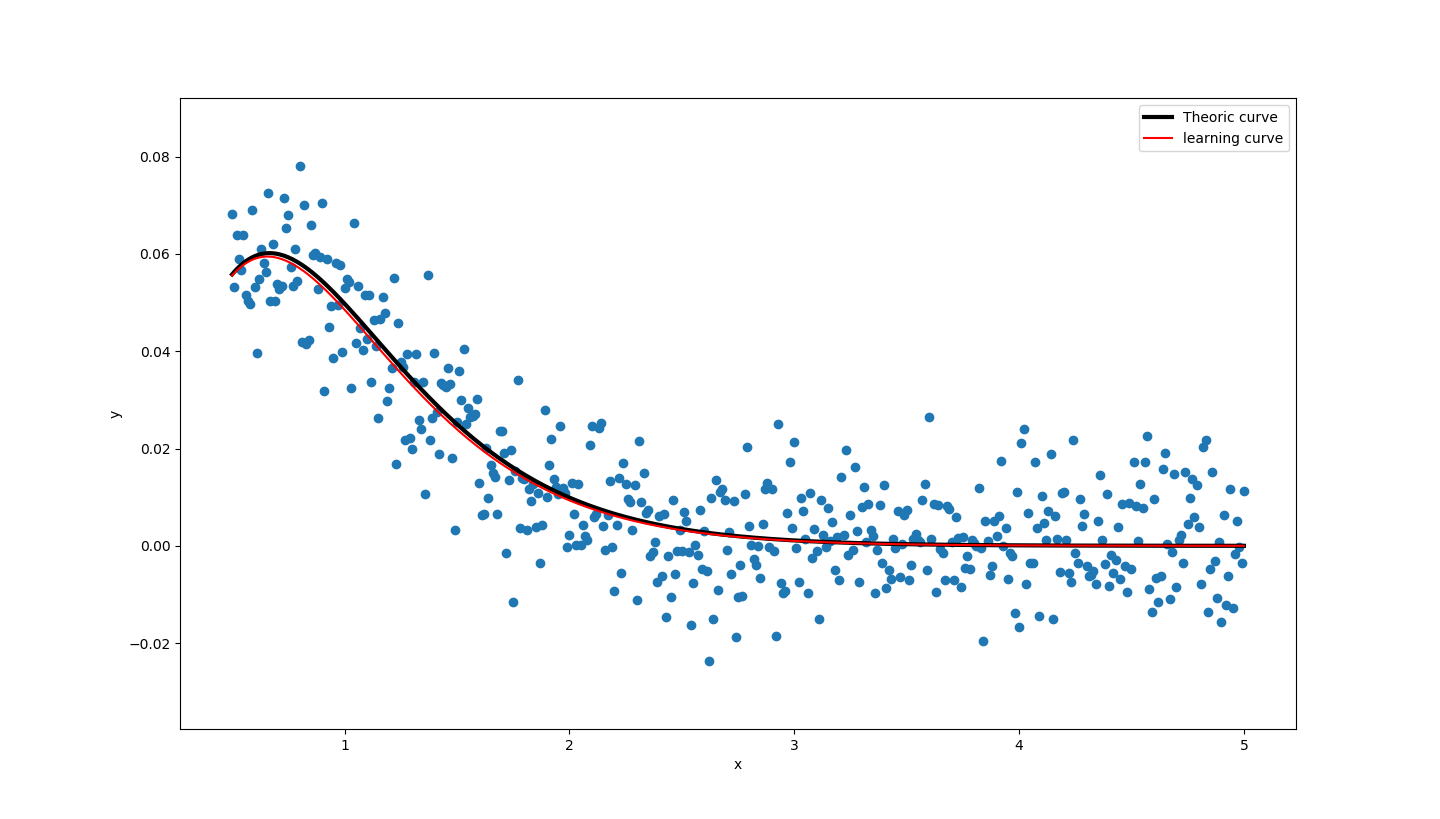
\includegraphics[width=0.7\textwidth]{Q15.png}
\caption{Représentation du jeu de données et de la courbe théorique $g(x)= x^{a1}e^{-a2x}$ en noire et de la courbe issue des approximation de $a_1$ et $a_2$ e rouge.}
\label{FigQ12}
\end{figure}
 
 \textbf{\color{brick}5 .} Comme précédemment nous allons observer l'évolution de $\lambda$, de $|g|$ et de la fonction de coût au cours des itérations, pour $g(x)=x^{a1}e^{-a2x} $, $b=0.01$ avec un jeu de données de 100 points, et des paramètres initiaux tels que $a_{1|k=0}=1.5$ et $a_{2|k=0}=1.5$ . 
 
  \begin{figure}[H]
\centering
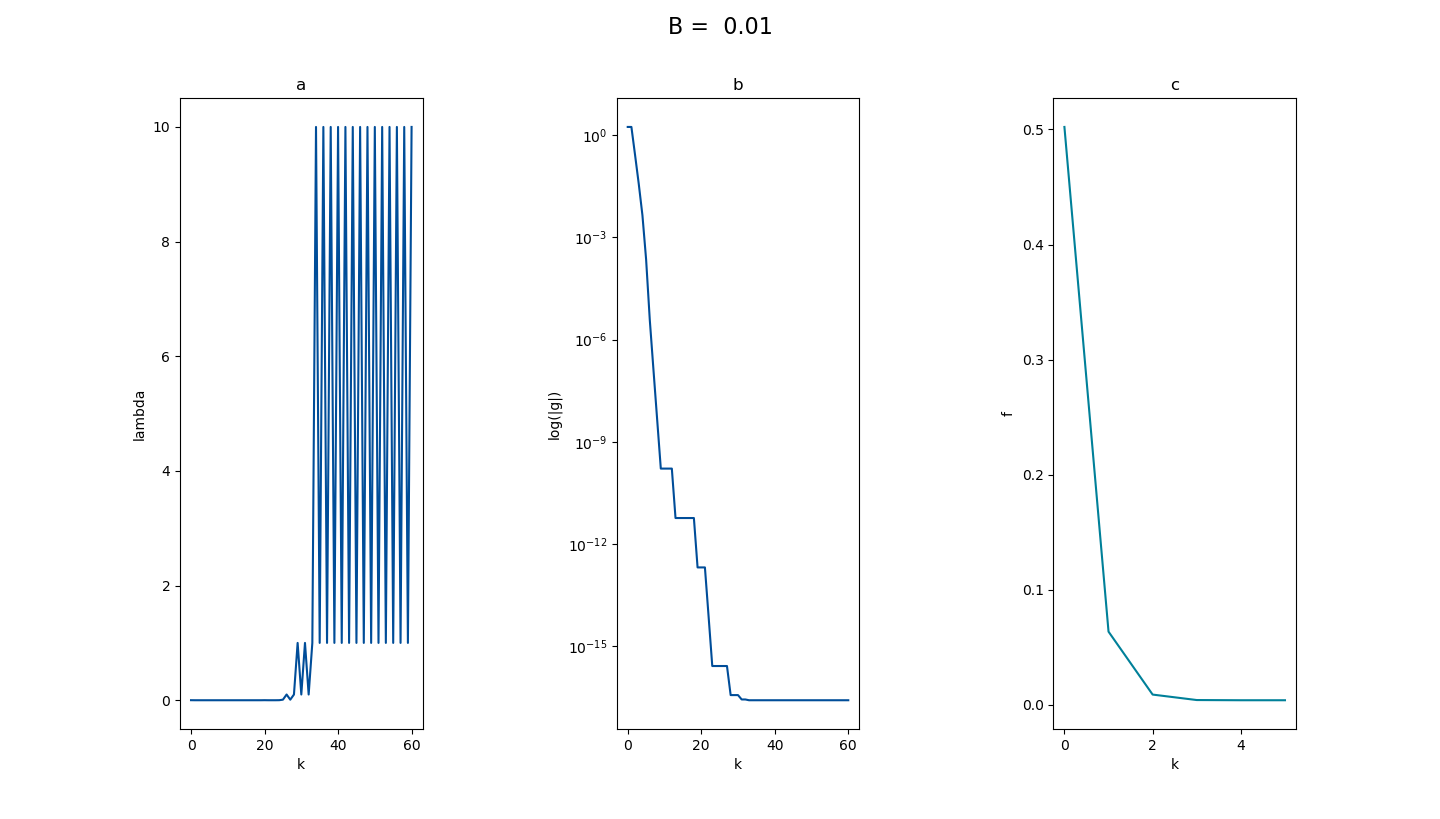
\includegraphics[width=0.8\textwidth]{Q16FFF.png}
\caption{\textbf{a)} Variation du $\lambda$ \textbf{b)} Variation du logarithme de $|g|$ \textbf{c)} variation de la fonction de coût (échelle réduite à cinq itérations)}
\label{FigQ12}
\end{figure}
 
Nous observons les mêmes tendances que dans le cas exponentielle, pour les différents paramètres testés. \\

Nous pouvons réitérer les analyses ci-dessus en faisant varier l'amplitude du bruit sur le jeu de données, nous testons notre modèle dans les mêmes conditions que précédemment pour des valeur de $b $

  
  \begin{figure}[H]
\centering
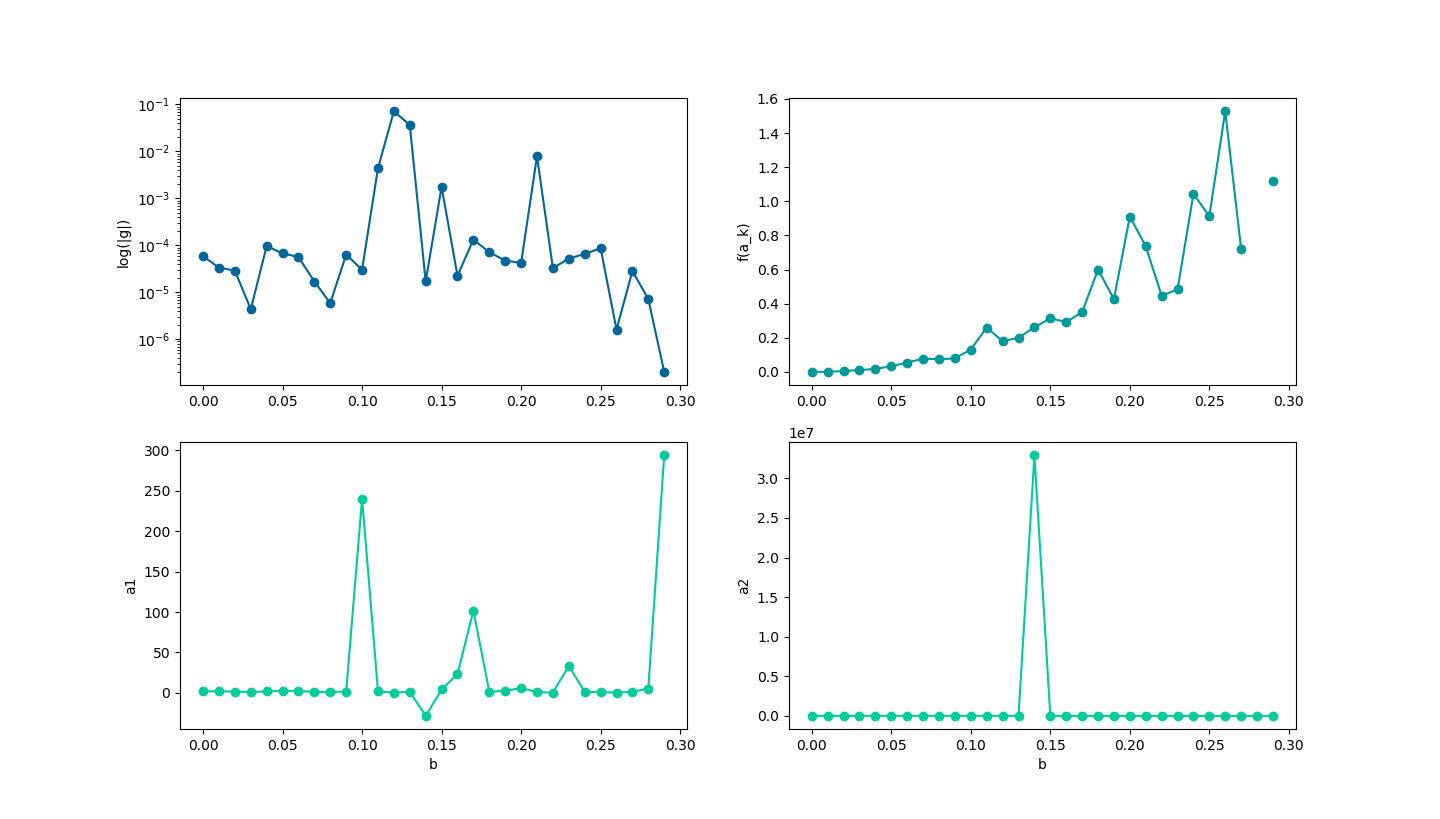
\includegraphics[width=1\textwidth]{Q17.png}
\caption{Évolution de $|g|$ de la fonction de coût, de $a_1$ et de $a_2$ en fonction du nombre d'itérations  )}
\label{FigQ12}
\end{figure}
Pour $b\in [0,0.3]$ nous observons globalement les mêmes tendances que dans le cas 1; on a une oscillation de $|g|$ autour de valeurs proches de 0, augmentation de la SCE, et des approximations des paramètres vers les valeurs théoriques. Cependant pour une telle majeur d'erreur on obtient des données qui peuvent osciller à $\pm 0.5$ ce qui et extrêmement grand étant donné les valeur théorique de la fonction $g(x)$ dont le maximum est autour de $0.06$. Considérer de telles valeurs de bruits revient alors à considérer notre jeu de données comme étant parfaitement aléatoire un ajustement à un quelconque modèle est alors aberrants.\\
Nous retiendrons donc des valeur de bruits telles que $b<0.1$. On a alors les résultats suivants : 

  \begin{figure}[H]
\centering
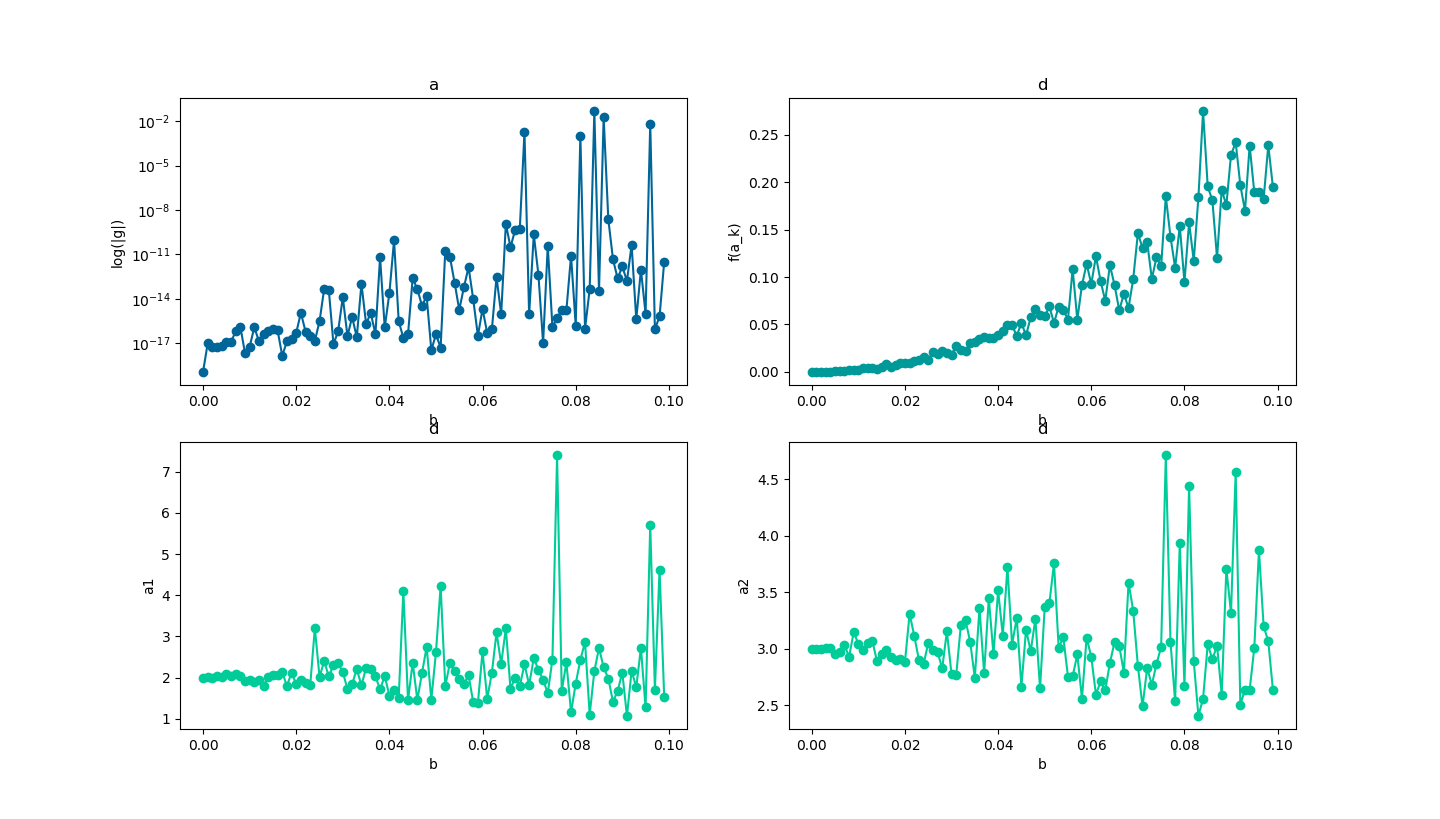
\includegraphics[width=1\textwidth]{Q17FFFF.png}
\caption{\textbf{a)} Évolution du $\log(|g|)$ \textbf{b)} Évolution de la fonction de coût \textbf{c)} Évolution de l'approximation de $a_1$  \textbf{d)} Évolution de l'approximation de $a_2$)}
\label{FigQ12}
\end{figure}

Pour des valeurs de bruits plus 'corrects' peut réinterpréter les résultats de façon identique au cas 1. De plus on observe que les solutions deviennent discutables dès $b = 0.02$
 \newpage
 \textbf{\color{brick}6 .} Nous pouons afficher les solutions pour les valeurs de bruit précédentes, le critère d'arrêt est fonction du nombre d'itération avec $k_{max}=100$ et de la norme du gradient avec $|g|_min= 0.001$ :
   \begin{figure}[H]
\centering
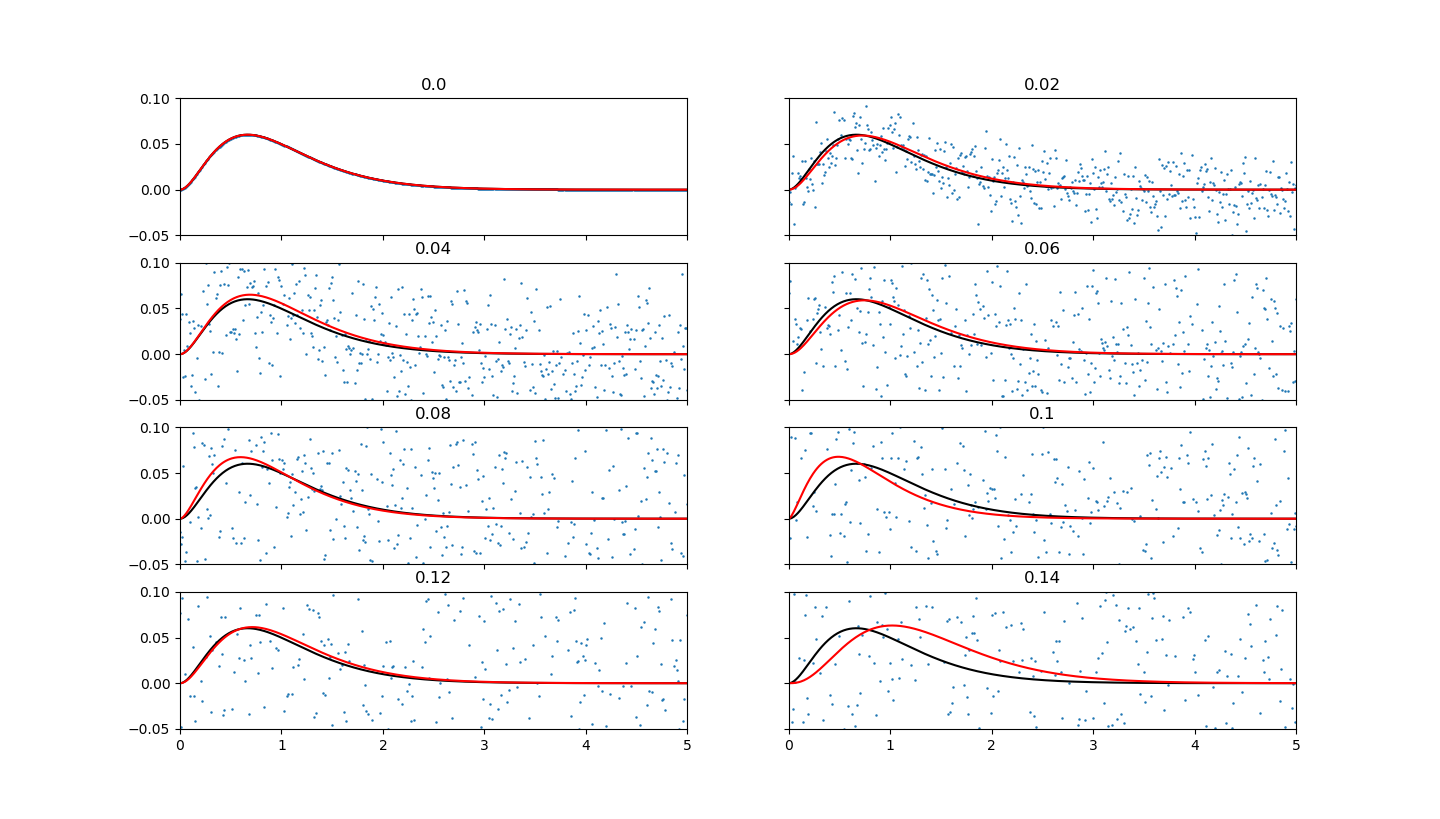
\includegraphics[width=1\textwidth]{Q18.png}
\caption{Les données aléatoirement tirés d'une lois normale centrée réduite pondérées par $b$ sont représentées par le nuage de points; la courbe théorique est représentée en noir et la courbe empirique pour un $b$ donné en rouge. )}
\label{FigQ12}
\end{figure}

Comme escompté l'augmentation du bruit induit un décalage entre le modèle théorique et empirique.

 \textbf{\color{brick}7 .}
\begin{center}
\fcolorbox{black}{lightgray}{
\begin{minipage}{\linewidth}
\textbf{Conclusion :} \\
L'algorithme de Levenberg Maquardt a été ici implémenté pour résolution du problème des moindre carrés dans le contexte de la régression non linéaire. Cette méthode fait la synthèse de deux méthodes d'optimisation vues précédemment, qui sont la descente de plus grande pente et la méthode de Newton. L'avantage de l'algorithme de Levenberg Maquardt est d'alterner les deux méthodes selon l'avancée du processus. Ainsi si l'estimation des paramètres est loin de leur valeur optimale la méthode de Newton sera privilégiée; on gagnera alors en efficacité et en rapidité; réciproquement si l'approximation des paramètres est proche de leur valeur optimale on utilisera la méthode de la descente, qui est quant elle de plus sûre.\\
On a ainsi observer une première phase où la méthode de Newton est privilégiée puis on passe ensuite à la méthode de gradient descente, avantde passer dans un éventuel régime alternatif.  
\end{minipage}}
\end{center}


   \end{document}
  